% !TeX root = ../BA_main_englisch.tex
% !TeX spellcheck = en_GB
We apply the methodology of Section \ref{n_5_ml} to the case of $\Delta \mathrm{T} = 1$ with $N=5$ drive and transducer qubits.
Contrary to $\Delta \mathrm{T} = 5$, the optimal system states\footnote{$\Tr{\rho_S^i \sigma_z} = 0$} cannot be reached from every point on the Bloch sphere, leading to a lower total work output following the protocol determined by the optimiser (Figure \ref{dt_dep}).

We train neural networks with the same hyperparameters as in Section \ref{n_5_ml}.
The performance of each network is listed in Table \ref{effdt1}.
We find that all networks outperform their $\Delta \mathrm{T} = 5$ counterparts, both in terms of efficiency and average work output.
In addition, the MSE score on the test data is lower, indicating that the predictions themselves are better.
There are two reasons for this occurrence: firstly, the predictive power of the networks is greater for $\Delta \mathrm{T} = 1$ than $\Delta \mathrm{T} = 5$, illustrated in Figure \ref{dt1box}.
Secondly, deviations between optimal and predicted transducer settings lead to a smaller difference between the respective system states as the evolution time is shorter.

\begin{table}[h]
	\centering
	\begin{tabular}{ c | c | c | c | c }
		Network Architecture & $\eta_{test} \ [\%]$ & $\mathrm{MSE}_{test}$  & $W_{test}$ & \# Parameters \\
		\hline
		FCANN        & 96.4 & 0.0265 & 1.61 & 8,086,020 \\
		Bidir. LSTM  & 97.4 & 0.0238 & 1.62 & 7,700,222 \\
		Unidir. LSTM & 70.1 & 0.0638 & 1.18 & 3,206,990 \\
	\end{tabular}
	\caption{Efficiencies $\eta$ and MSE loss on the test set for differing model architectures for $N=5, \Delta \mathrm{T} = 1$.}
	\label{effdt1}
\end{table}

For $\Delta \mathrm{T} = 1$, all models beat the locally optimised average $W_{lo} = 1.14$.


\begin{figure}
	\centering
	\begin{subfigure}{0.35\textwidth}
		\centering
		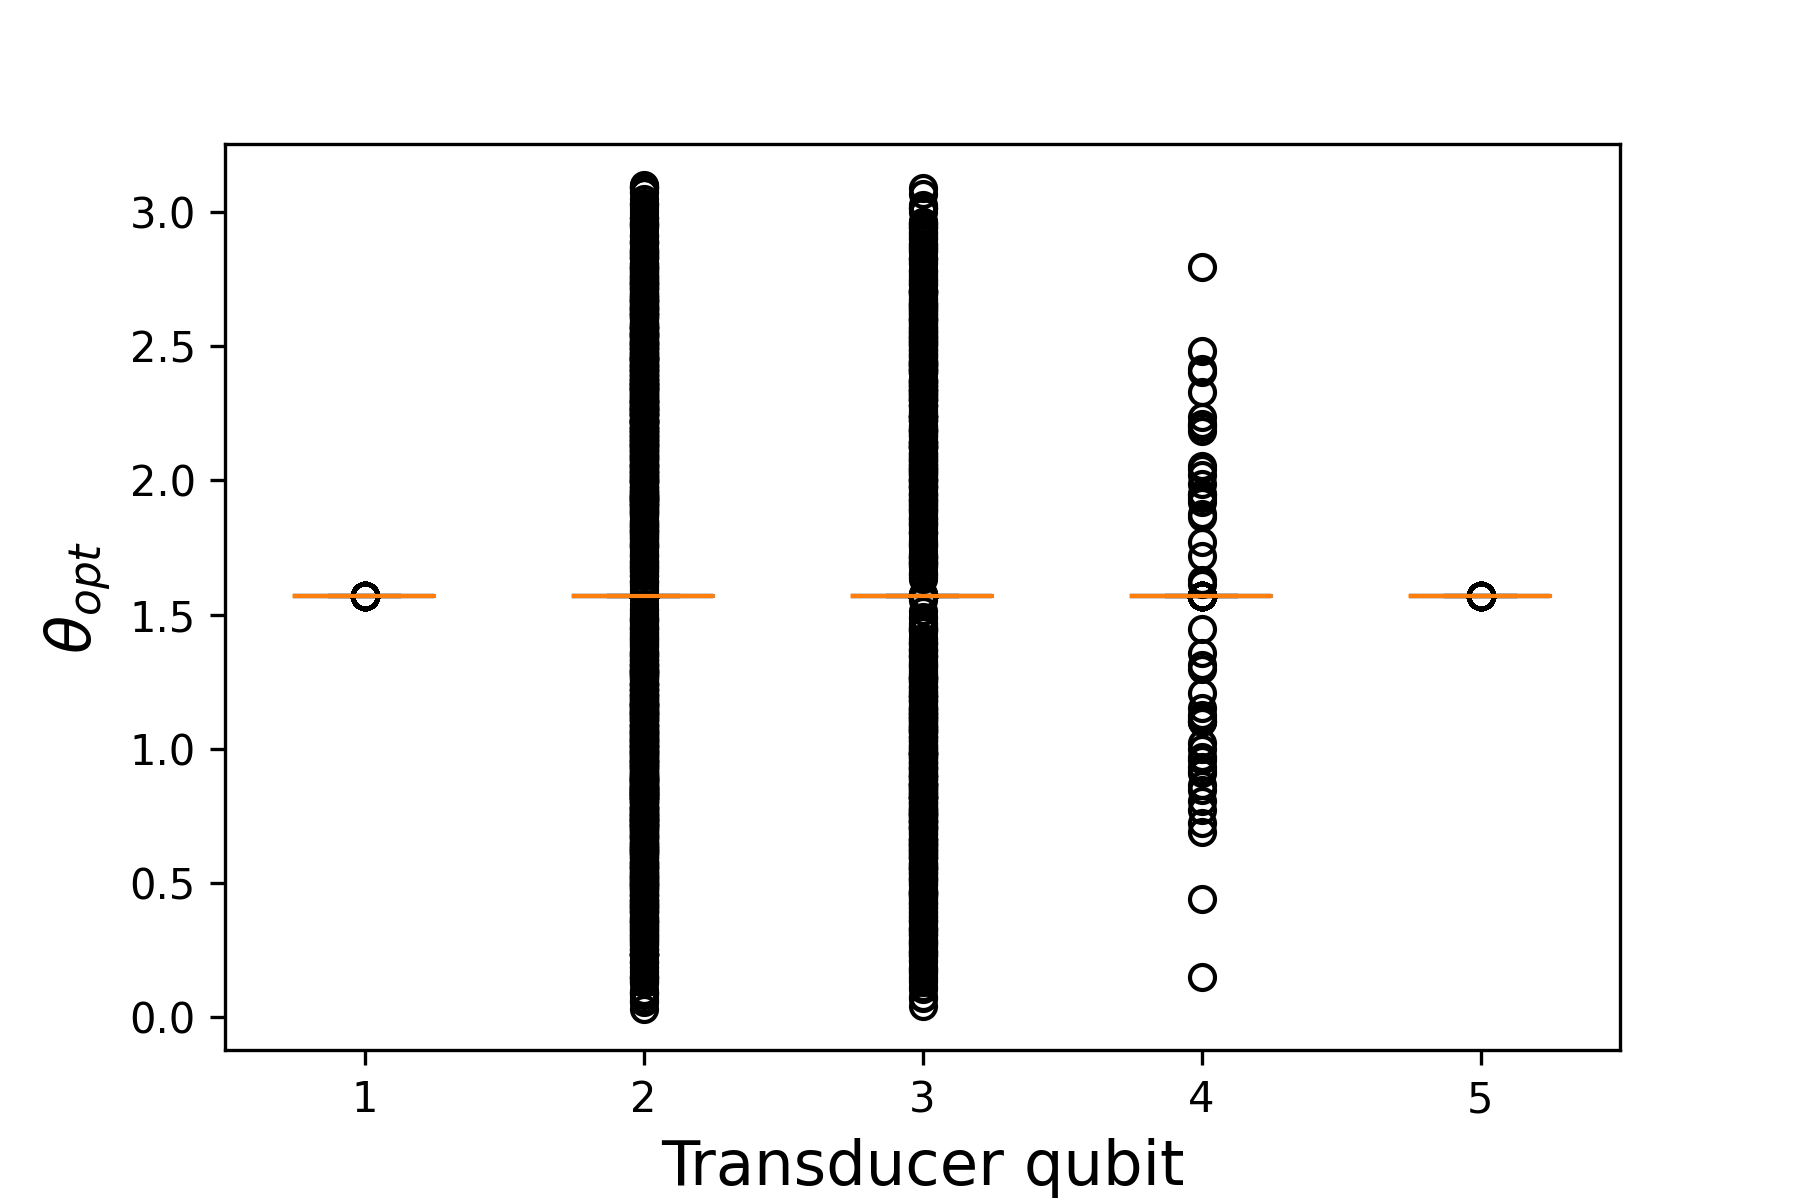
\includegraphics[width=\textwidth]{img/theta_opt_box_dt_12}
		\subcaption{$\theta^n_{\text{opt}}$}
	\end{subfigure}
	\begin{subfigure}{0.35\textwidth}
		\centering
		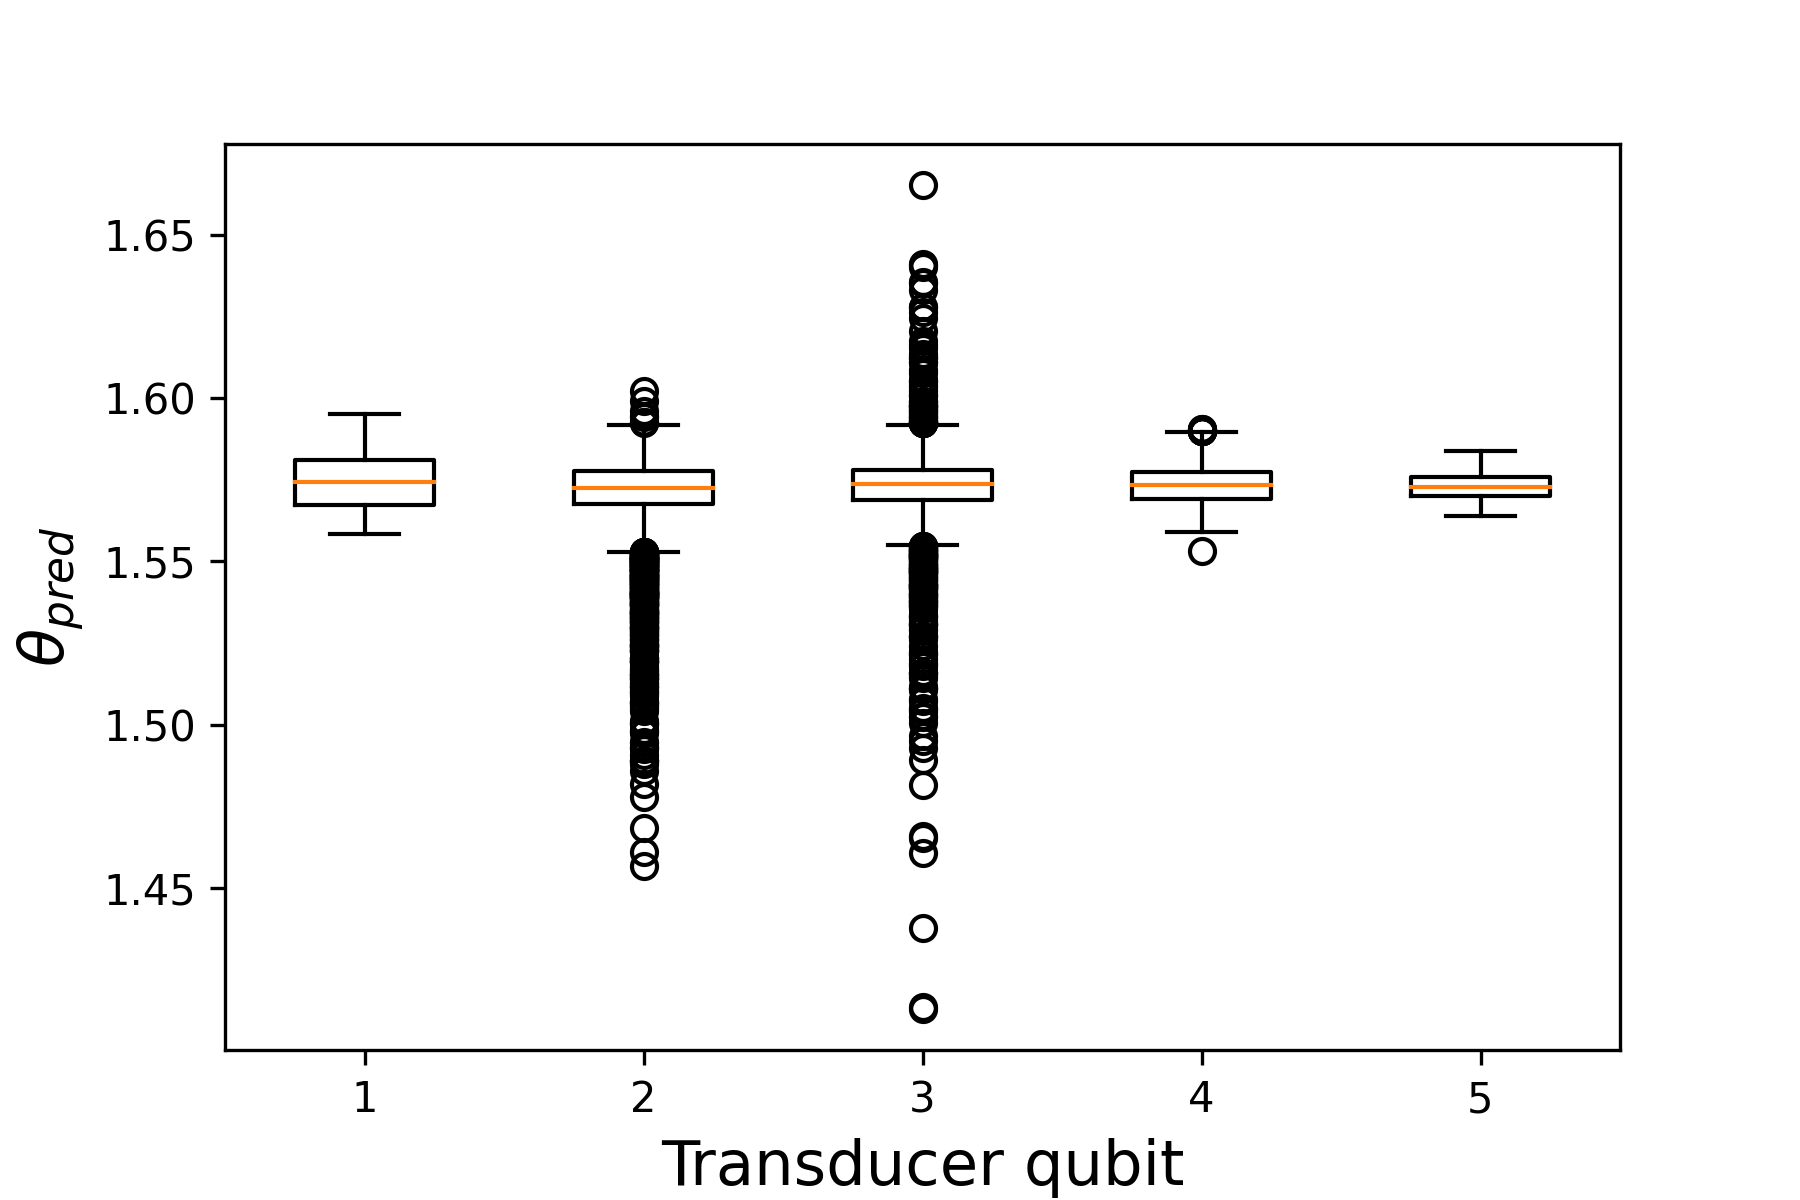
\includegraphics[width=\textwidth]{img/theta_pred_box_dt_12}
		\subcaption{$\theta^n_{\text{pred}}$}
	\end{subfigure}
	\begin{subfigure}{0.35\textwidth}
		\centering
		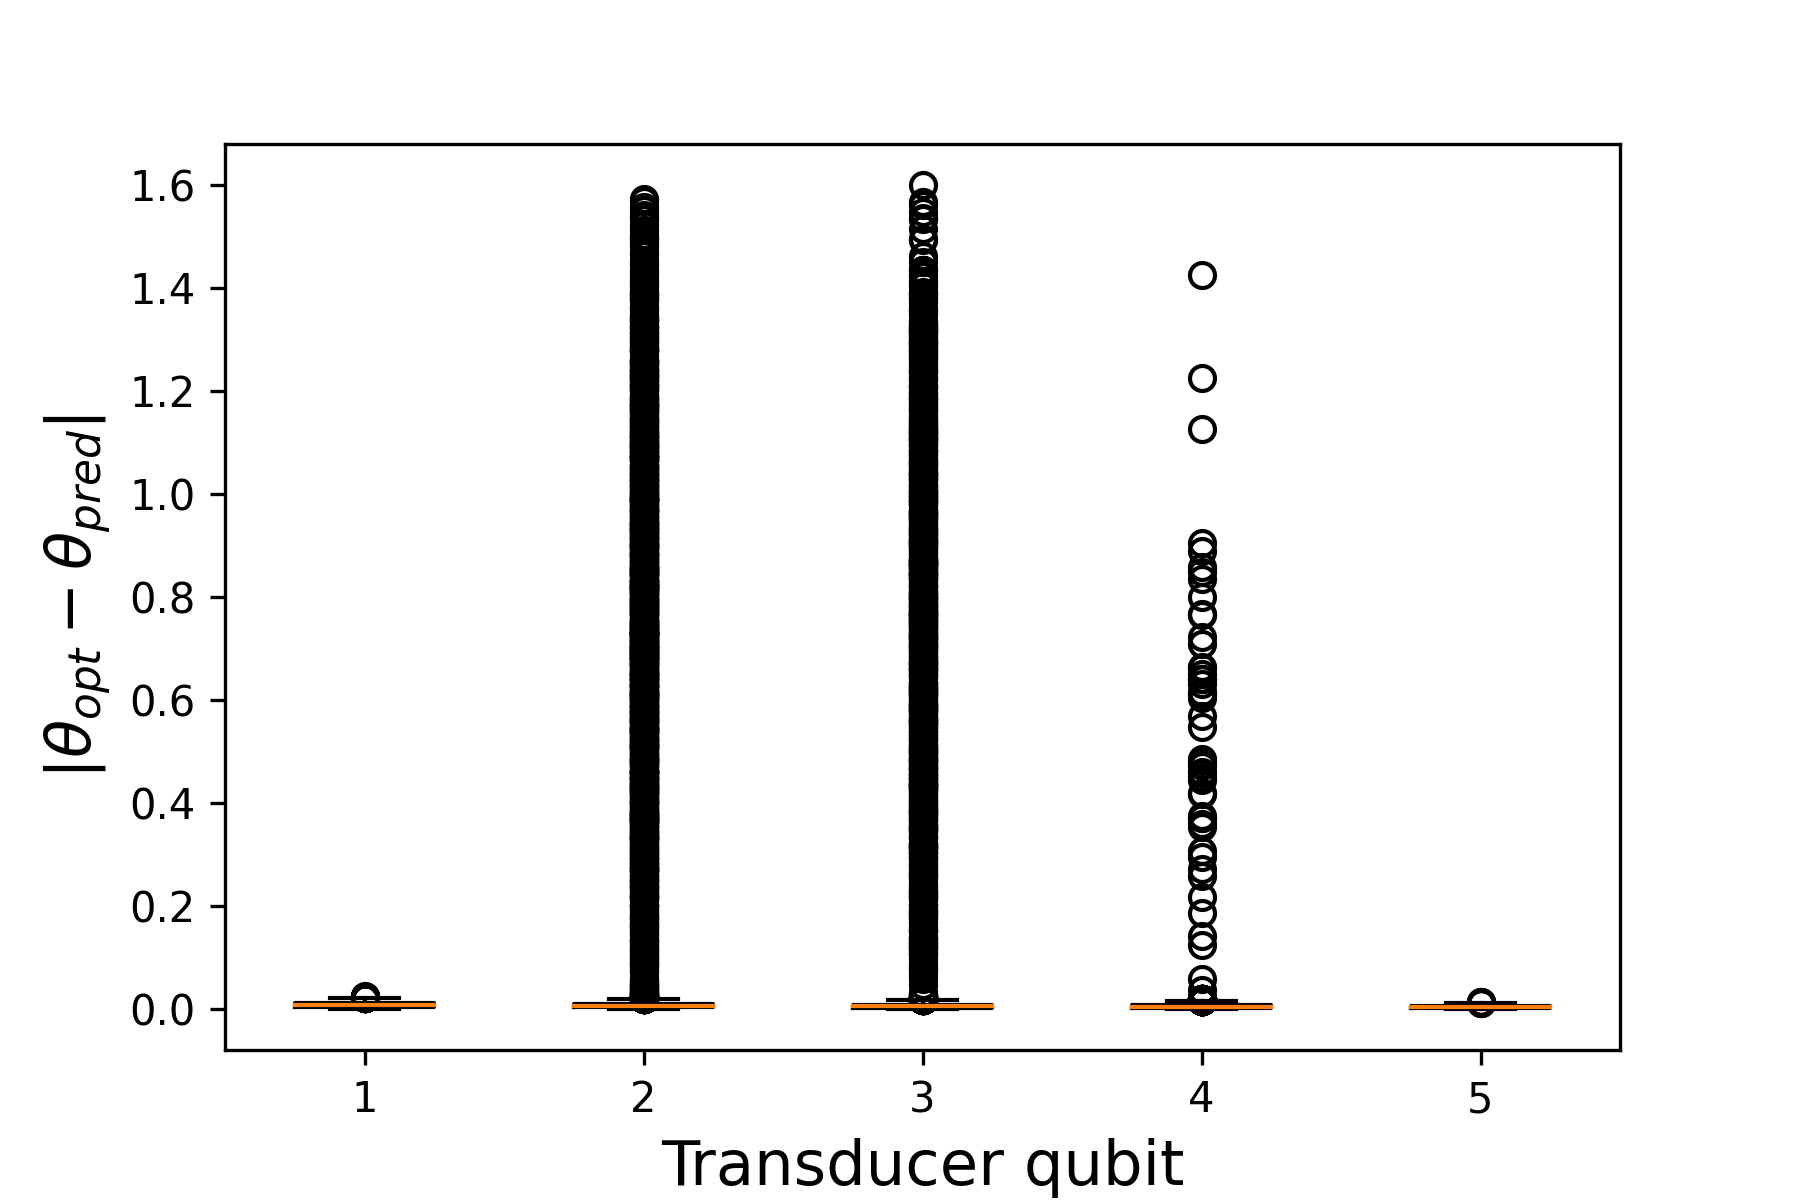
\includegraphics[width=\textwidth]{img/delta_theta_box_dt_12}
		\subcaption{$|\theta^n_{\text{opt}} - \theta^n_{\text{pred}}|$}
	\end{subfigure}
%	\begin{subfigure}{0.32\textwidth}
%		\centering
%		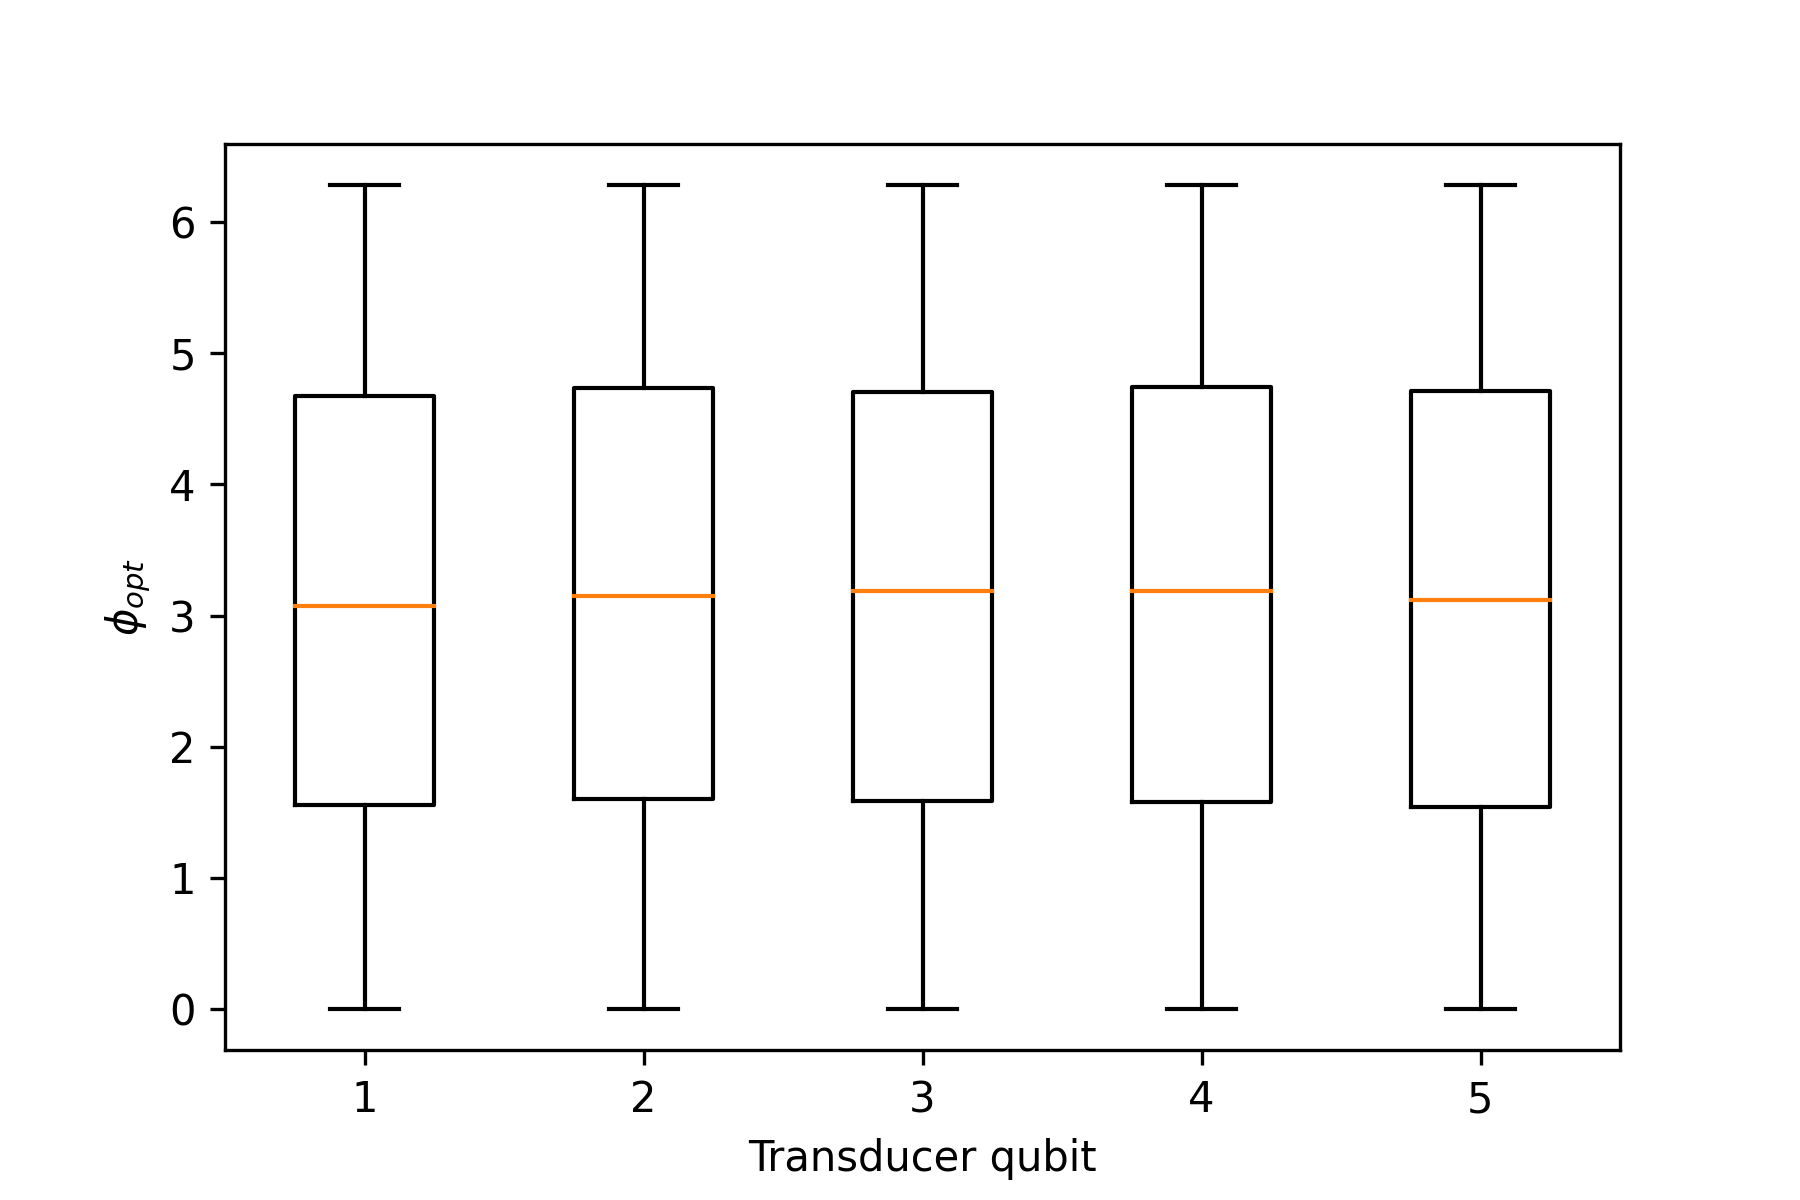
\includegraphics[width=\textwidth]{img/phi_opt_box_dt_1}
%	\end{subfigure}
%	\begin{subfigure}{0.32\textwidth}
%		\centering
%		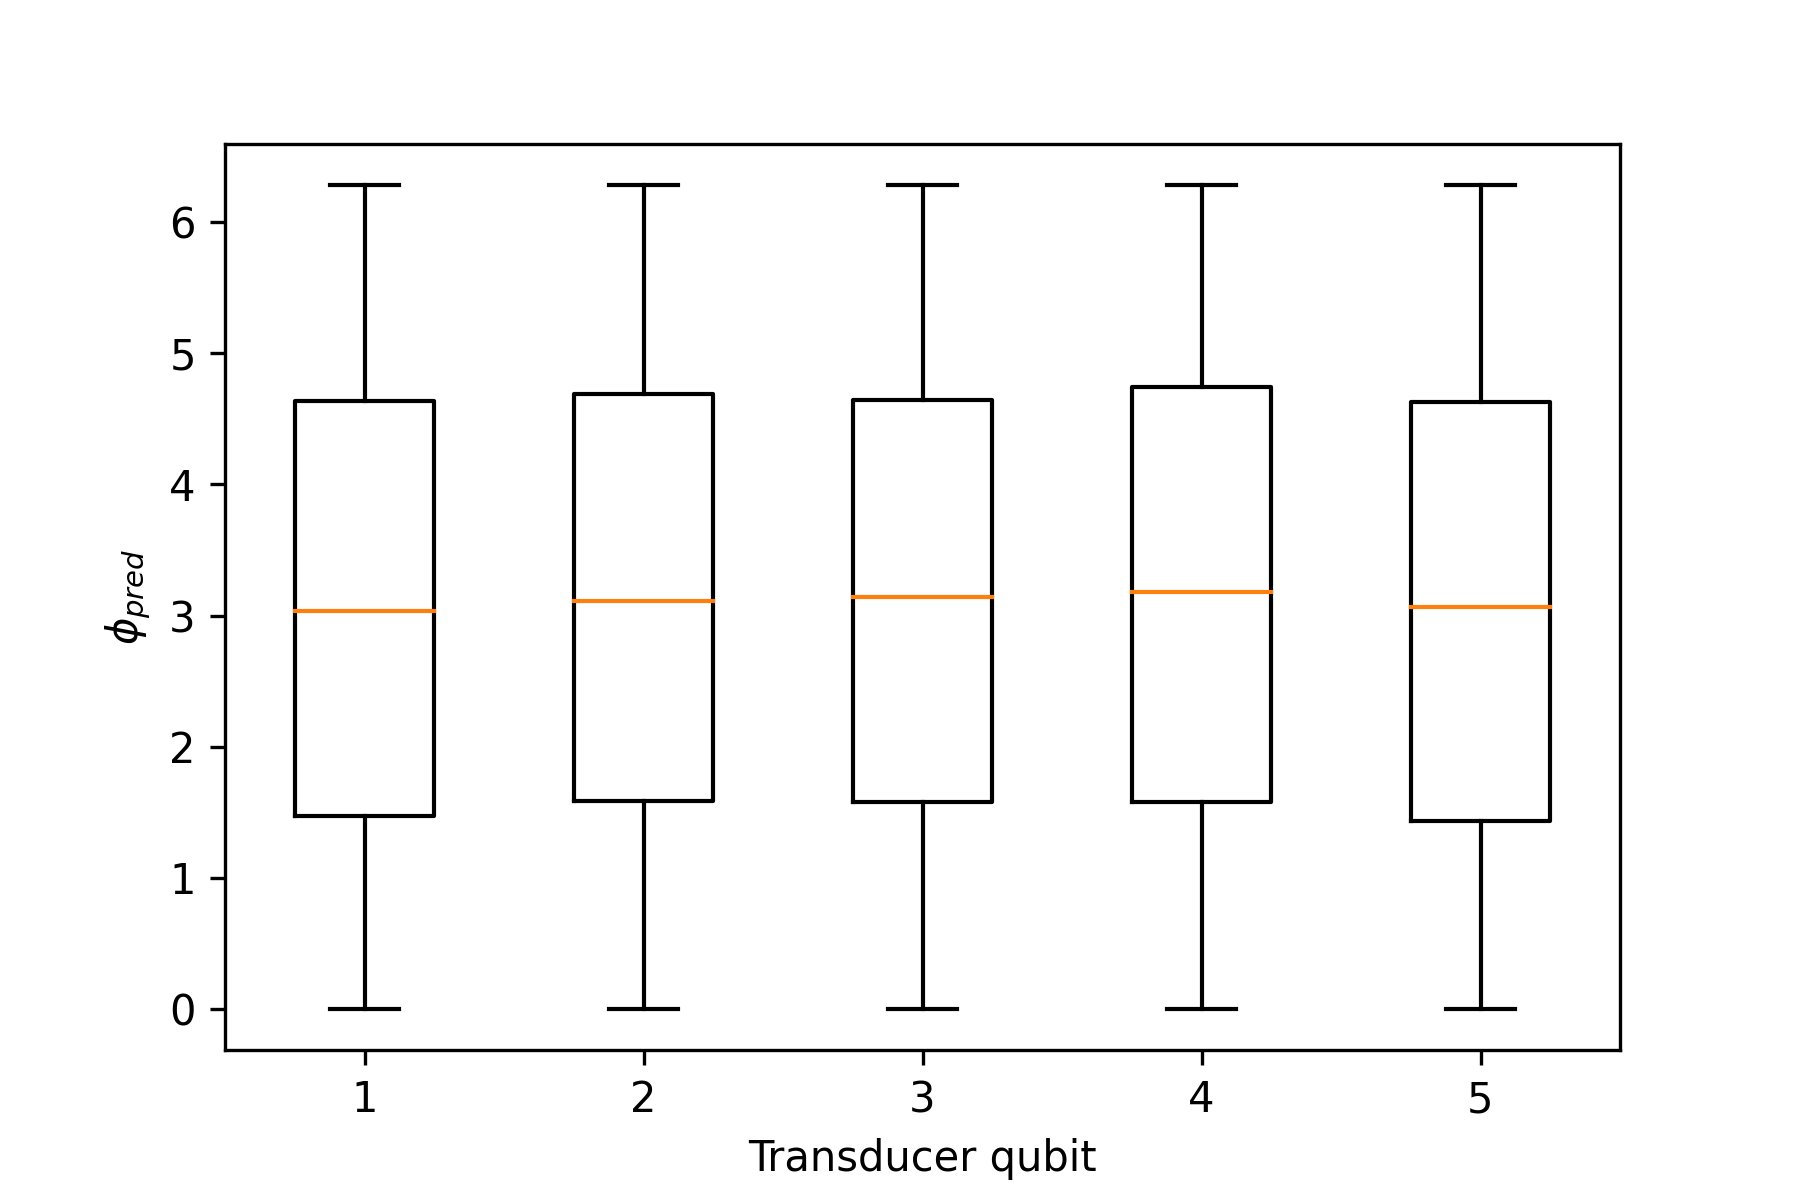
\includegraphics[width=\textwidth]{img/phi_pred_box_dt_1}
%	\end{subfigure}
	\begin{subfigure}{0.35\textwidth}
		\centering
		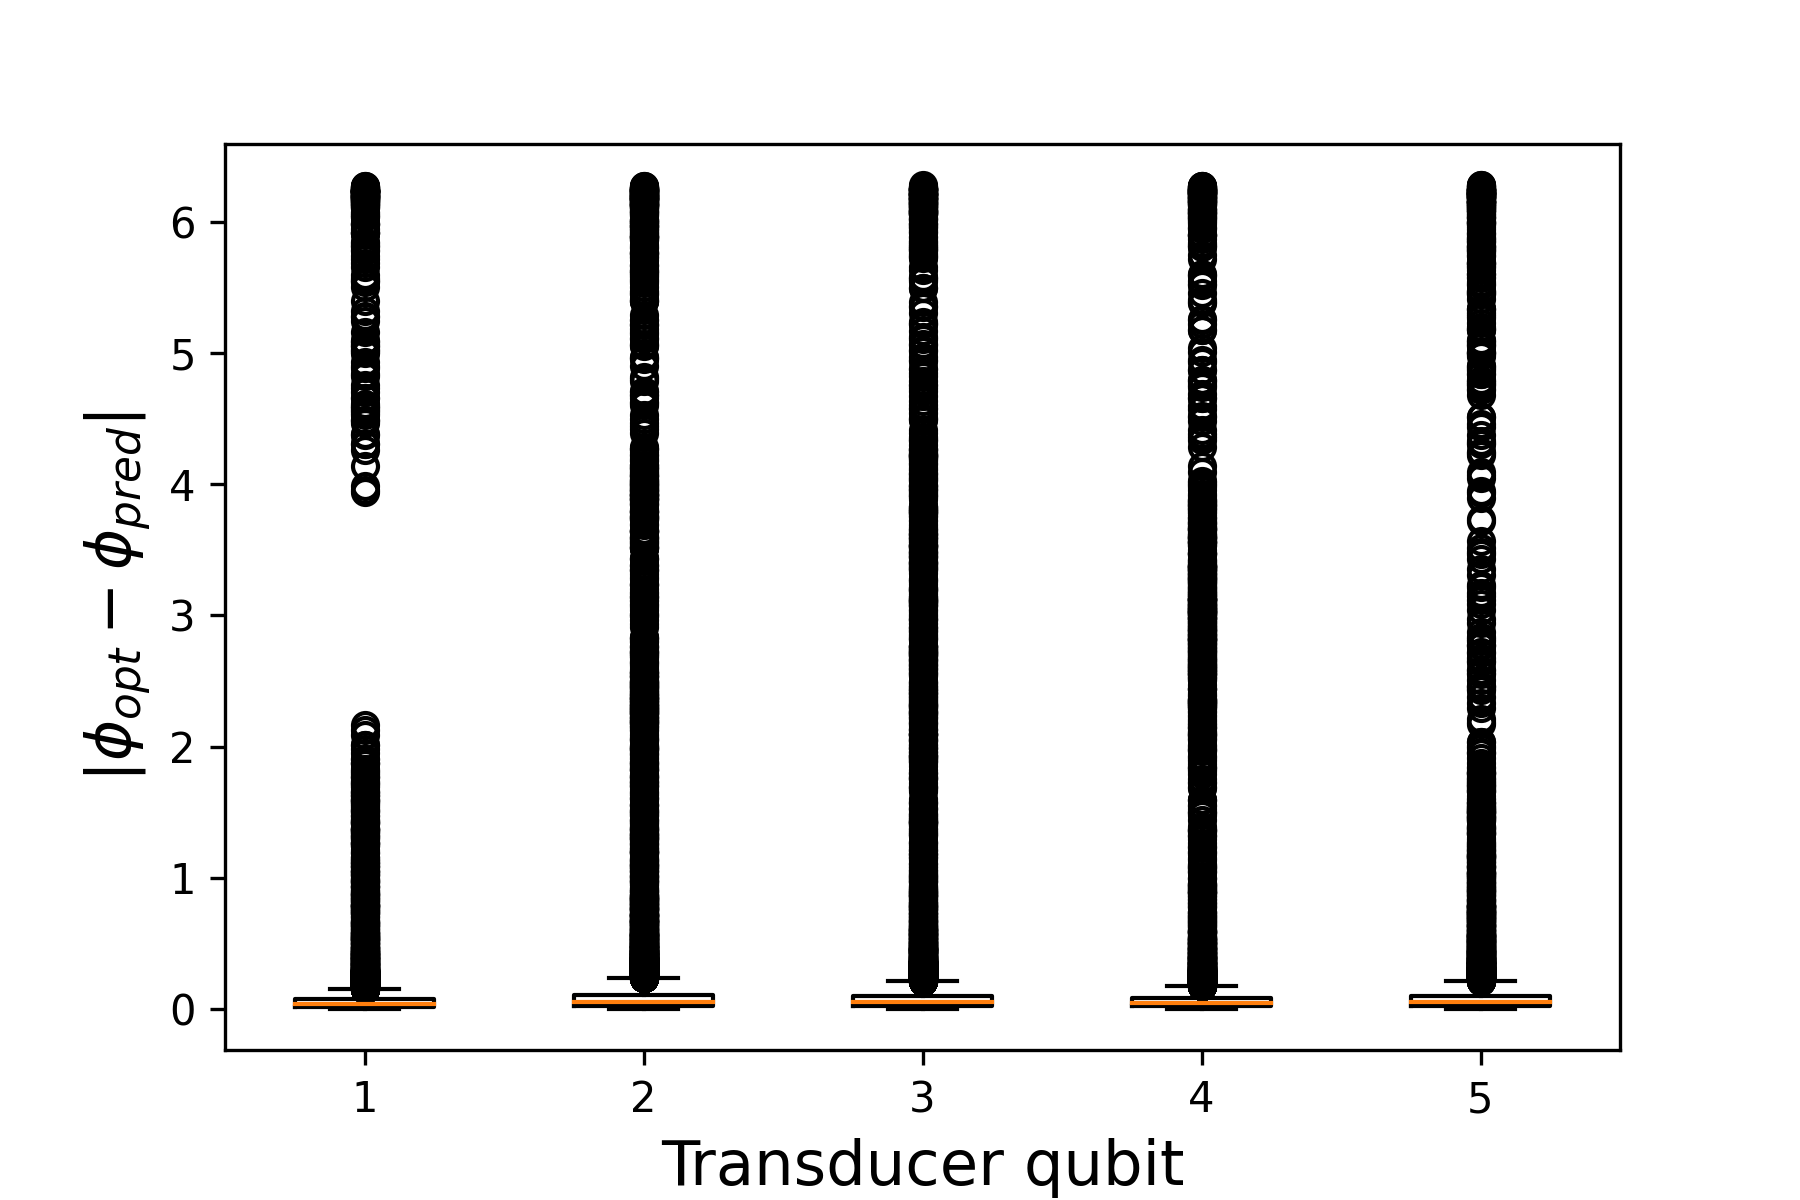
\includegraphics[width=\textwidth]{img/delta_phi_box_dt_12}
		\subcaption{$|\phi^n_{\text{opt}} - \phi^n_{\text{pred}}|$}
	\end{subfigure}
	\caption{We plot the performance of the bidirectional LSTM for $\Delta \mathrm{T} = 1$. Unlike the optimum for the longer switching time, $\theta_T^n = \frac{\pi}{2}$ for a majority of the central three qubits as well. Again, predicted and optimal $\phi^n_T$ are distributed equally and thus we do not plot them here.}
	\label{dt1box}
\end{figure}

We illustrate the difference between $\Delta \mathrm{T} = 1$ and $\Delta \mathrm{T} = 5$ in Figure \ref{blochsdt15}.

\begin{figure}
	\centering
	\begin{subfigure}{0.85\textwidth}
		\centering
		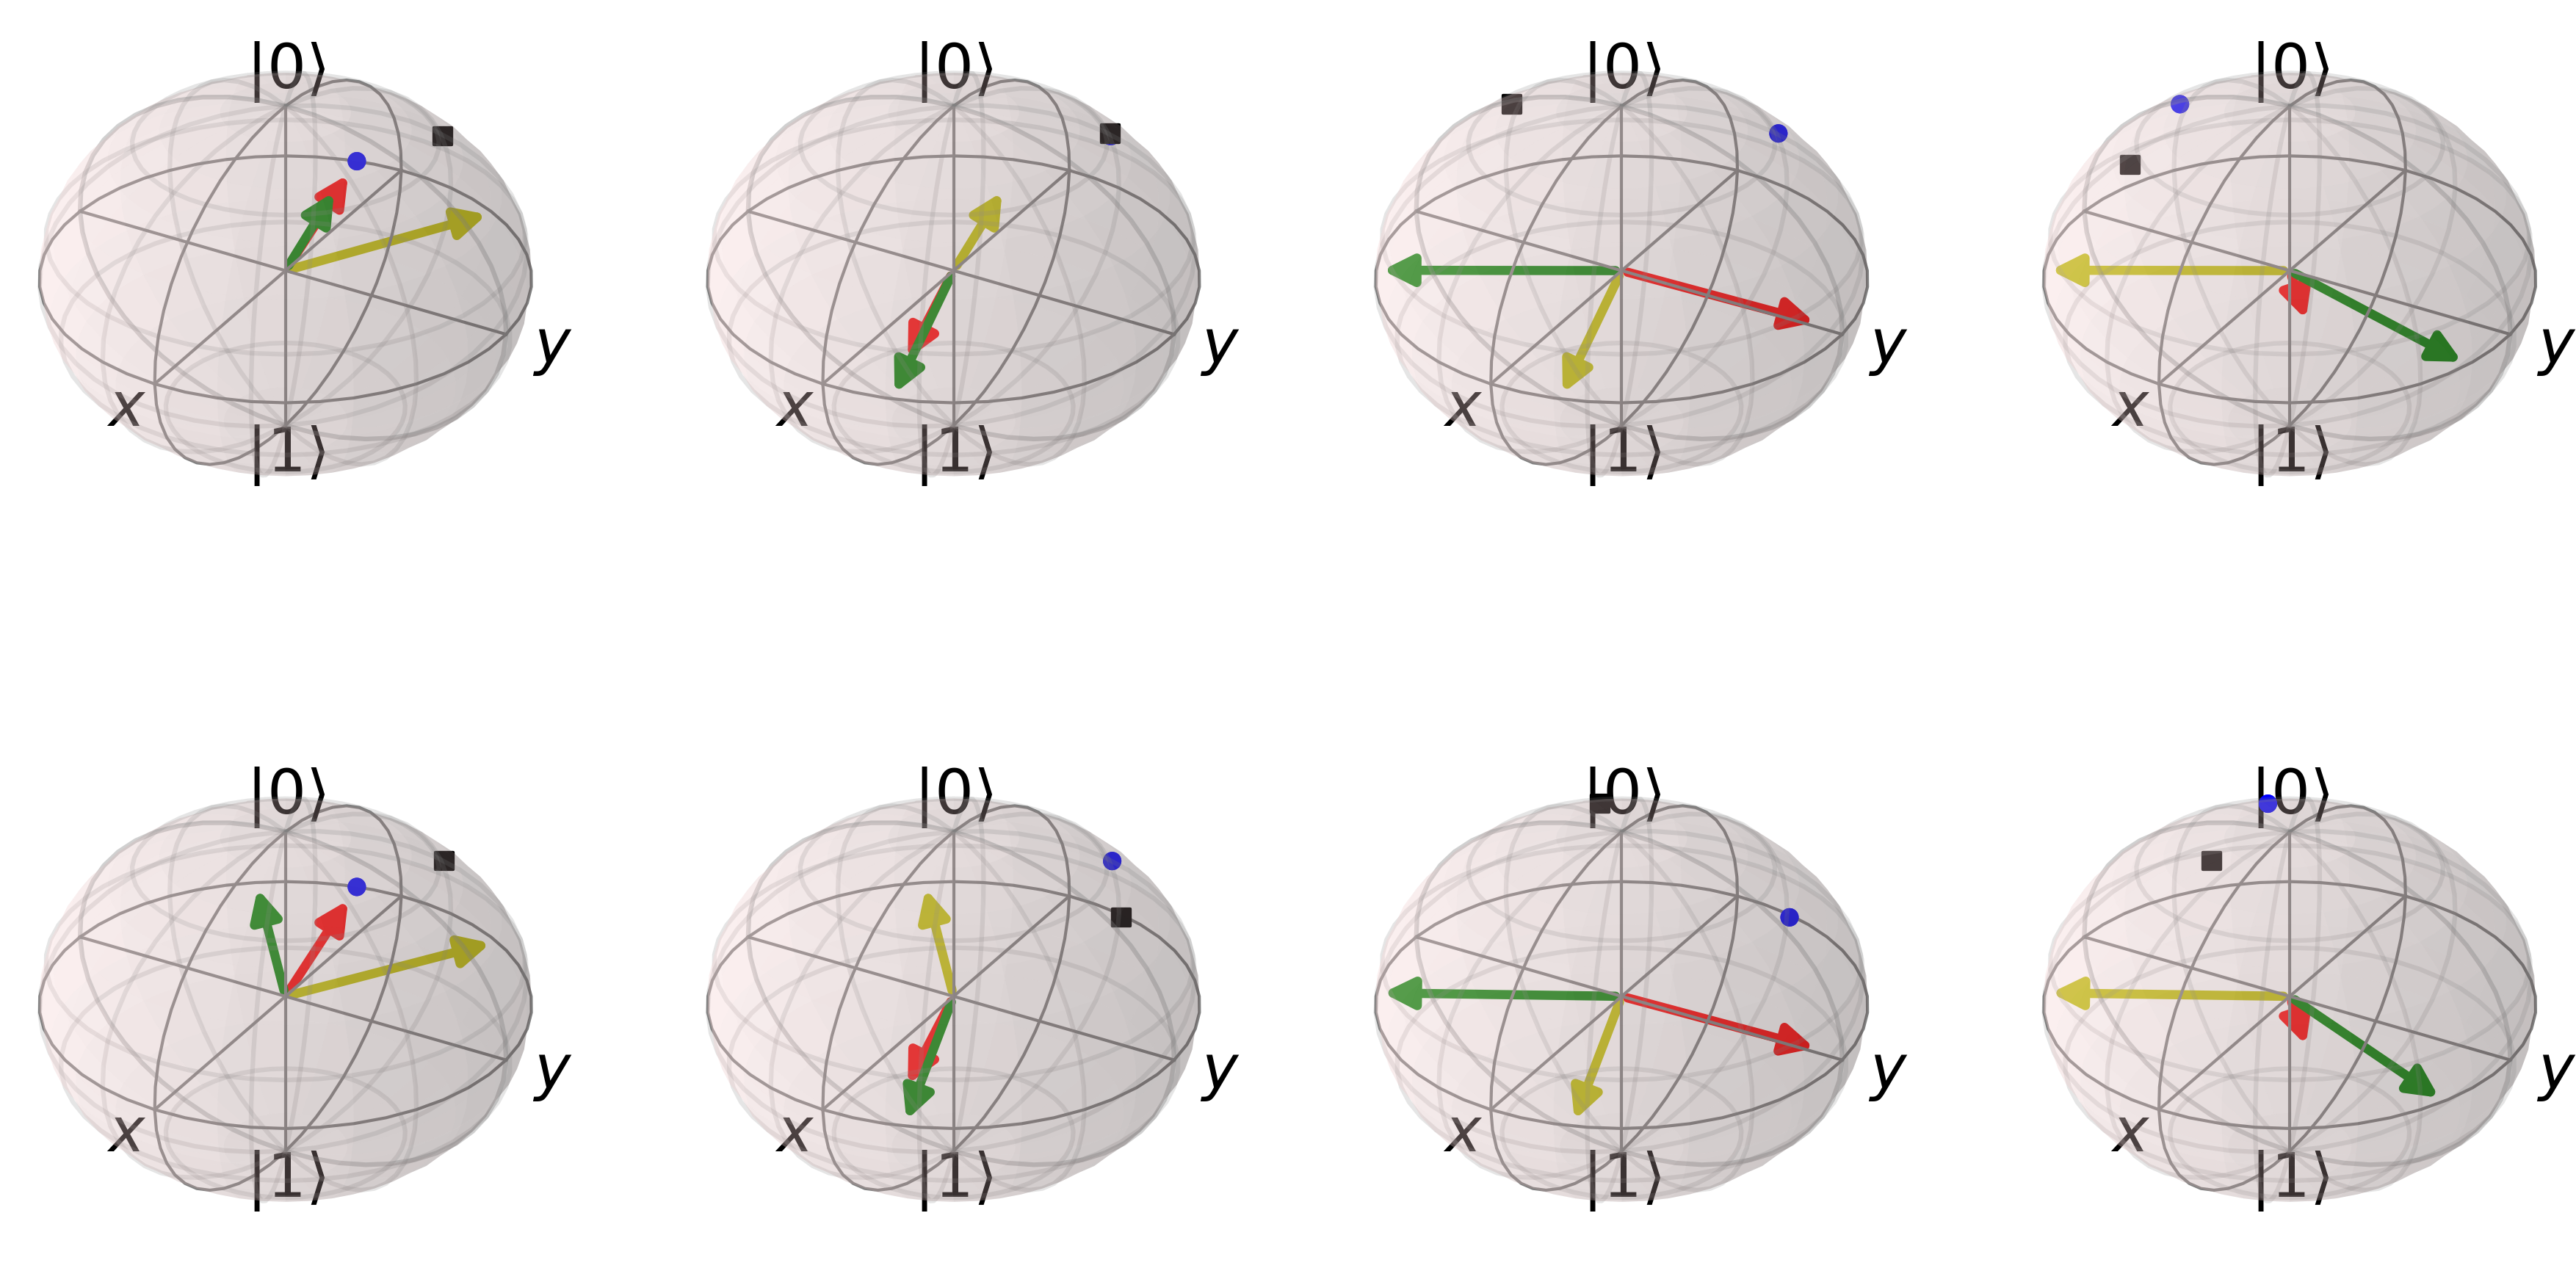
\includegraphics[width=\textwidth]{img/bloch_comp_1_crop}
		\caption{$\Delta \mathrm{T} = 1: W_{opt} = 1.40, W_{pred} = 1.32$}
		\label{}
	\end{subfigure}
	\begin{subfigure}{0.85\textwidth}
		\centering
		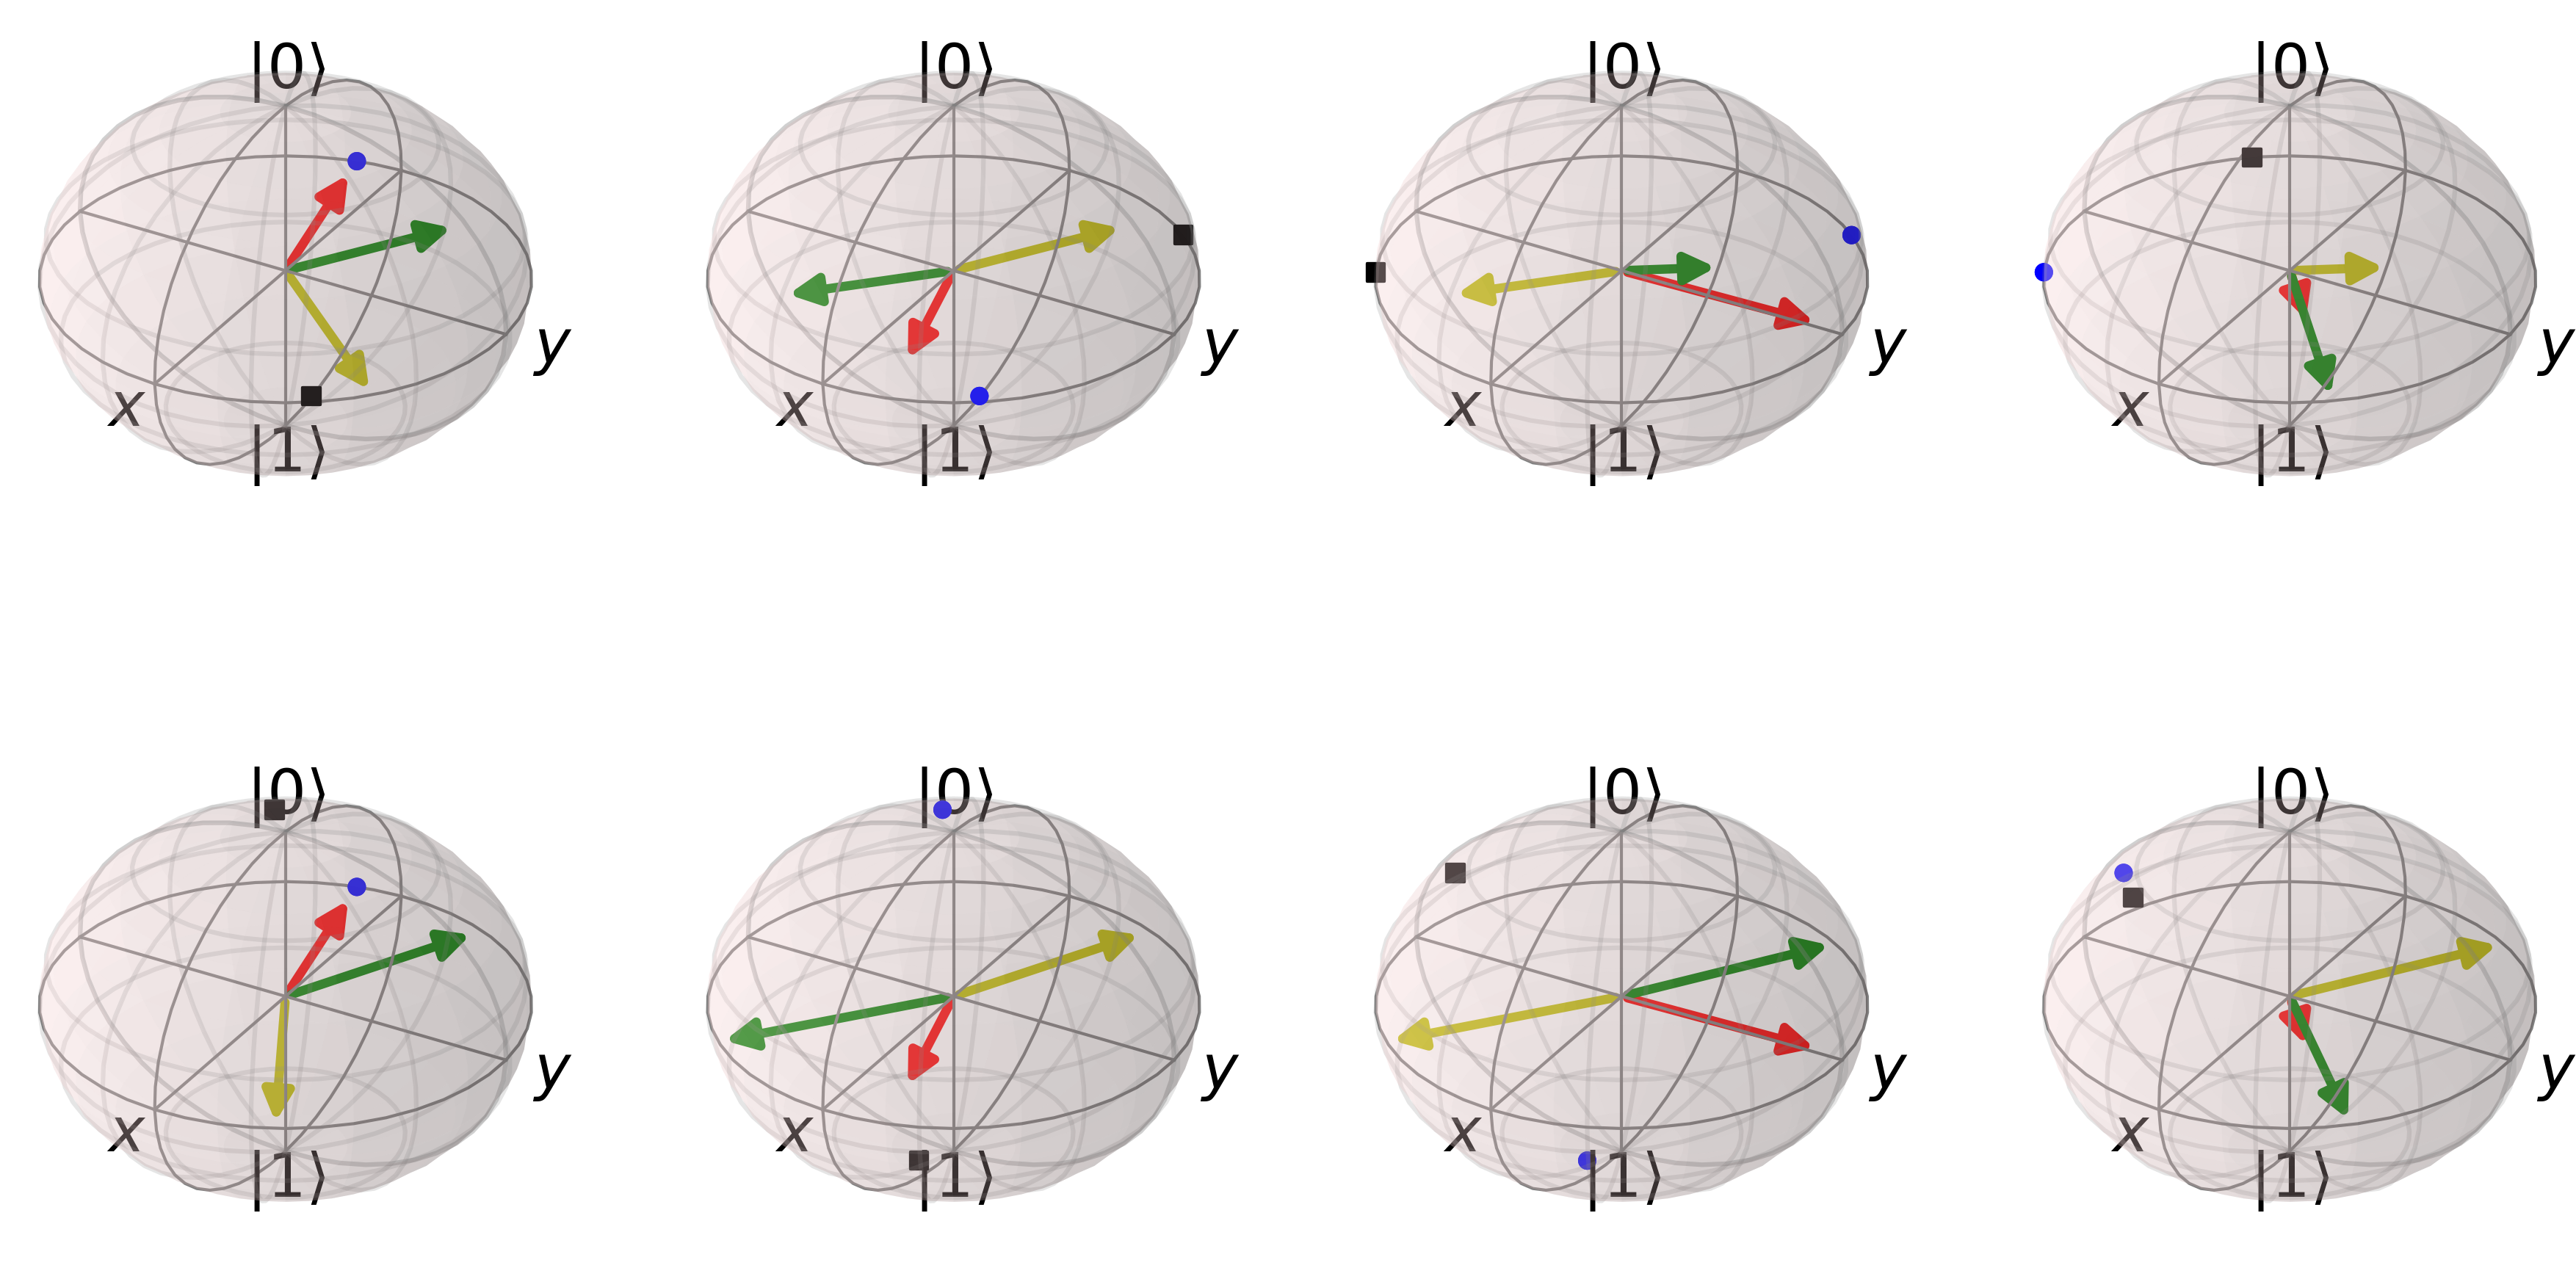
\includegraphics[width=\textwidth]{img/bloch_comp_5_crop}
		\caption{$\Delta \mathrm{T} = 5: W_{opt} = 2.42, W_{pred} = 0.57$}
		\label{}
	\end{subfigure}
	\caption{We plot the optimal (top row) and predicted (bottom row) system state and transducer settings for the bidirectional LSTM, using the same representation as in Figure \ref{n_5_blochs}, for $\Delta \mathrm{T} = 1$ (a) and $\Delta \mathrm{T} = 5$ (b). The drive sequence is the same in all rows and is a sample from the test set. For $\Delta \mathrm{T} = 1$, the optimal system state, where $\Tr{\rho_S^i \sigma_z} = 0$, cannot be reached.}
	\label{blochsdt15}
\end{figure}